\documentclass[letterpaper,10pt]{IEEEtran}
\usepackage{geometry}                % See geometry.pdf to learn the layout options. There are lots.
\geometry{letterpaper}                   % ... or a4paper or a5paper or ... 
%\geometry{landscape}                % Activate for for rotated page geometry
%\usepackage[parfill]{parskip}    % Activate to begin paragraphs with an empty line rather than an indent
\usepackage{graphicx}
\usepackage{amssymb}
\usepackage{epstopdf}
\usepackage{multicol}
\usepackage{tikz}
\usetikzlibrary{calc}
\usepackage{mathptmx}
\usepackage{amsmath}
\usepackage{algpseudocode}
\usepackage{url}
\newcommand{\BigO}[1]{\ensuremath{\operatorname{O}\bigl(#1\bigr)}}



\DeclareGraphicsExtensions{.pdf,.png,.jpg}
\usepackage{wrapfig}

% Spacing stuff
\usepackage[cm]{fullpage}
\addtolength{\voffset}{-.5in}
\setlength{\topmargin}{0pt}
\setlength\footskip{0pt}
\setlength{\parskip}{0cm}
%\setlength{\parindent}{1em}
%\usepackage[compact]{titlesec}
%\titlespacing{\section}{0pt}{2ex}{1ex}
%\titlespacing{\subsection}{5pt}{1ex}{2ex}
%\titlespacing{\subsubsection}{0pt}{0.5ex}{0ex}

\title{Vine Project}
\author{
Donnie Smith (donnie.smith@gatech.edu) \\
Kyle Harrigan (kwharrigan@gatech.edu) 
}	
\date{November 29, 2012}                                           % Activate to display a given date or no date


\markboth{CS 6491 Fall 2012, Project 4}{}
\begin{document}

\bibliographystyle{IEEEtran}

\maketitle

 %\begin{abstract}
 
 
 %\end{abstract}
 
%\section{Introduction
%}
%\IEEEPARstart{I}{nitially} 

%\section{Results}

%\bibliography{cs6491}

\section{Project Description}

Given a triangle mesh, we are to build a pseudo-Hamiltonian cycle of vertices (meaning we only visit each edge once).   This cycle is used to essentially divide the triangle mesh into two parts.  These parts are colored differently to indicate which of the two sets they belong to.  Given this subdivision, we pick a root and simulate a vine growing along each of these paths as a breadth first invasion. 

\section{Heuristic Approximation to Hamiltonian Cycle }

Due to the computational complexity of calculating a true Hamiltonian cycle, the following algorithm is implemented. 

{\tiny
\begin{verbatim}
void makeCycle(int s) {
    int c = s;                                               // start at the seed corner s
    phc_vm[v(n(c))] = true
    phc_vm[v(p(c))] = true;                // mark vertices as visited
     do {
     if (!phc_vm[v(c)]) phc_vm[v(c)] = phc_tm[t(c)] = true; // invade c.t
      else if (!phc_tm[t(c)]) c = o(c);                      // go back one triangle
      c = r(c);                                              // advance to next ring edge on the right
    } while (c != o(s));                                     // until back at the beginning
    }
\end{verbatim}
}

\section{Breadth First Invasion of Vine}

In order to progressively invade the two submeshes (inside and outside the cycle), two triangles (one inside and one outside) are initially marked visible, and their indices are added to a list.
Before each subsequent frame is rendered, for each triangle in the list, all non-visible neighbors of those triangles which are on the same side of the cycle (again, inside or outside) are marked visible, and added to a new list.
The new list is then swapped with the old list.

In this way, the submeshes are invaded at one triangle per path per frame, and as paths in the submeshes branch, each path is invaded simultaneously.

\begin{figure}[!h]
\centering
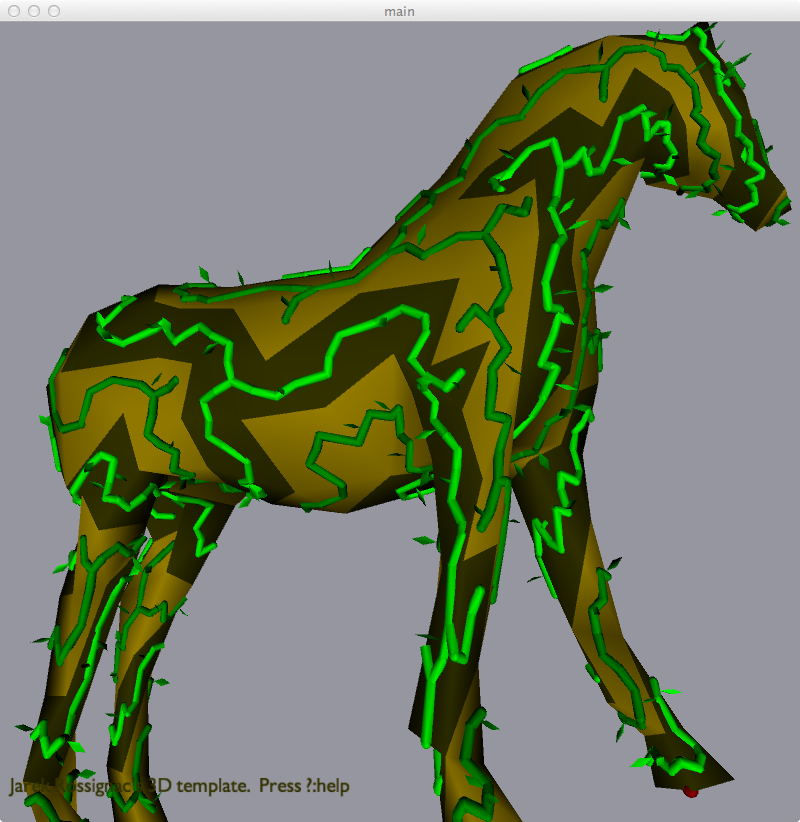
\includegraphics[width=3in]{data/vine}
\caption{Example of Vine around Horse}
\label{fig_angle}
\end{figure}

\section{Showing the vine}

For each triangle, there are four control points: the center of the triangle, defined as the average of the three vertices, and one at the middle of each edge.

As the triangles are invaded, vines are drawn only on the invaded triangles, and only from the center control points to the edge control points corresponding to neighbor triangles on the same side of the cycle.

The vine segments between triangle centers are drawn as cylinders using  \verb+TRIANGLE_STRIP+.
Each vine segment is represented by some number of radial triangle strips.
In our examples, we used 12 radial segments in order to form the vine, which resulting in a fairly smooth shape that is visually pleasing.

At the intersection of each vine segment, a smooth interface must be formed so that the vine looks continuous.
For this purpose, a sphere was drawn at each intersection.

The leaves are pseudo-randomly placed according to the index of the corner to the left of the edge control point being drawn.
Each segment has a one in four chance of containing a leaf, and the angle formed by the leaf stalk with respect to the triangle is uniformly distributed between 0 and $\pi$ radians in increments of $\frac{\pi}{10}$.
The vine leaves are drawn using \verb+TRIANGLE_FAN+.

\section{Future Work}

Improve drawing of leaves
Speed


\begin{IEEEbiography}[{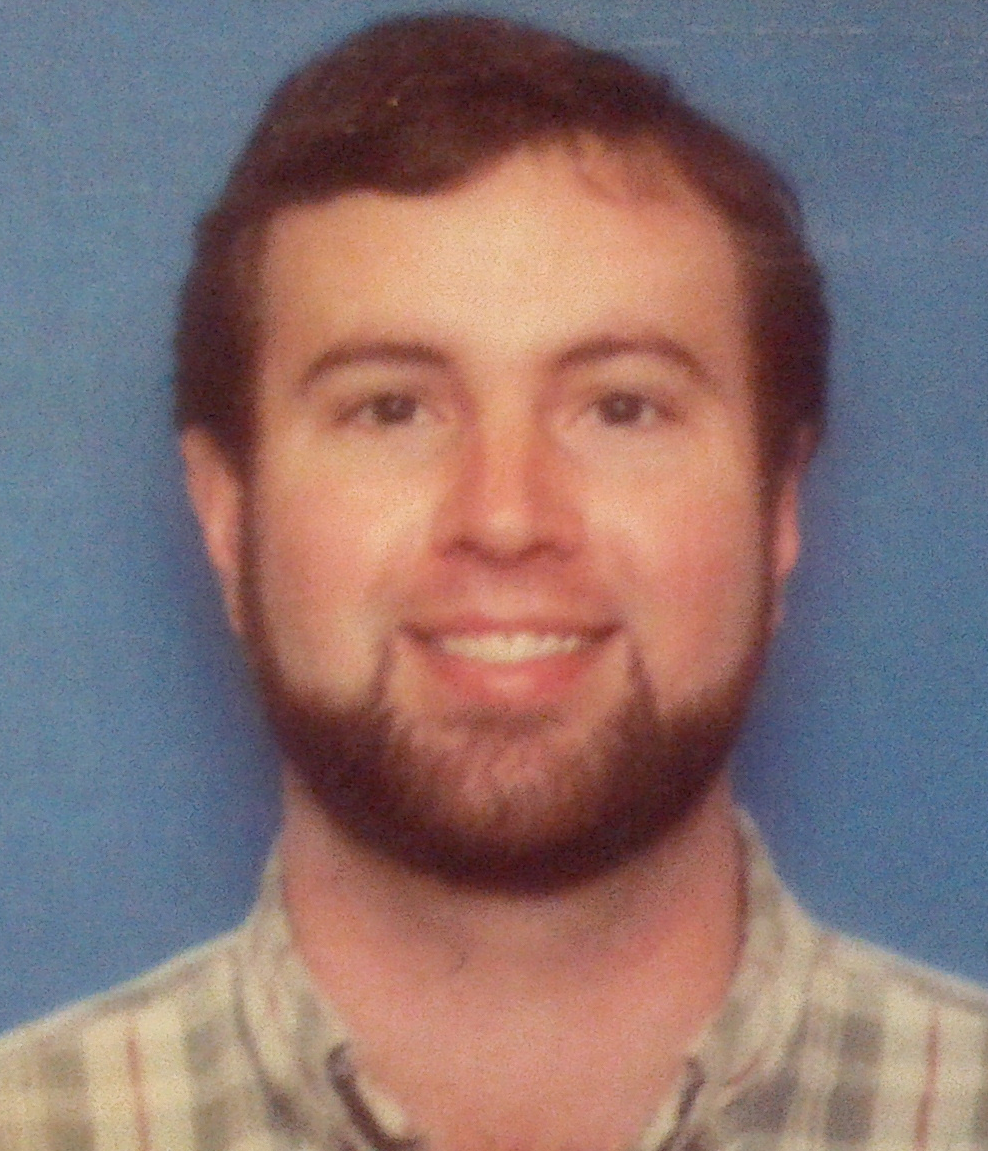
\includegraphics[width=1in,height=1.25in,clip,keepaspectratio]{data/dsmith.png}}]{Donnie Smith} donnie.smith@gatech.edu
\end{IEEEbiography}

\begin{IEEEbiography}[{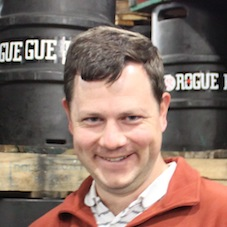
\includegraphics[width=1in,height=1.25in,clip,keepaspectratio]{data/kwharrigan.jpg}}]{Kyle Harrigan} kwharrigan@gatech.edu
\end{IEEEbiography}
\end{document}
